\documentclass{beamer}

\usefonttheme{professionalfonts} % using non standard fonts for beamer
\usefonttheme{serif} % default family is serif

\usepackage{enumitem}
\setitemize{label=\usebeamerfont*{itemize item}%
  \usebeamercolor[fg]{itemize item}
  \usebeamertemplate{itemize item}}

\usepackage{hyperref}
\usepackage{booktabs}
\usepackage{xfp}
\usepackage{graphicx}
\def\Put(#1,#2)#3{\leavevmode\makebox(0,0){\put(#1,#2){#3}}}
\usepackage{colortbl}
\usepackage{tikz}
\usepackage{amssymb}
\usepackage{enumerate}
\usepackage{arydshln}
\usepackage{algorithm}
\usepackage{algpseudocode}
\usepackage{subcaption} %to have subfigures available

\usepackage[absolute,overlay]{textpos}

\colorlet{lightred}{red!25}
\colorlet{lightgreen}{green!25}
\beamertemplatenavigationsymbolsempty

\newcommand\blfootnote[1]{%
  \begingroup
  \renewcommand\thefootnote{}\footnote{#1}%
  \addtocounter{footnote}{-1}%
  \endgroup
}

\makeatletter

%% Textclass specific LaTeX commands.
\newcommand\makebeamertitle{\frame{\maketitle}}%
\AtBeginDocument{%
  \let\origtableofcontents=\tableofcontents
  \def\tableofcontents{\@ifnextchar[{\origtableofcontents}{\gobbletableofcontents}}
  \def\gobbletableofcontents#1{\origtableofcontents}
}
%% User specified LaTeX commands.
\usetheme{Malmoe}
\useoutertheme{infolines}
\addtobeamertemplate{headline}{}{\vskip2pt}
\setbeamercovered{transparent}

\title[PFlock report]{PFLOCK Report}
\author[AC]{Andres Calderon}
\institute[UCR]{University of California, Riverside}
\makeatother

%%%%%%%%%%%%%%%%%%%%%%%%%%%%%%%%%%%%%%
%% Main document
%%%%%%%%%%%%%%%%%%%%%%%%%%%%%%%%%%%%%%
\begin{document}
\makebeamertitle
\newif\iflattersubsect

\AtBeginSection[] {
    \begin{frame}<beamer>
    \frametitle{Outline} 
    \tableofcontents[currentsection]  
    \end{frame}
    \lattersubsectfalse
}

\AtBeginSubsection[] {
    \begin{frame}<beamer>
    \frametitle{Outline} 
    \tableofcontents[currentsubsection]  
    \end{frame}
}

\begin{frame}{PSI stages...}{Small dense dataset (100 points, $\varepsilon$=1, $\mu$=3)}
    \centering
    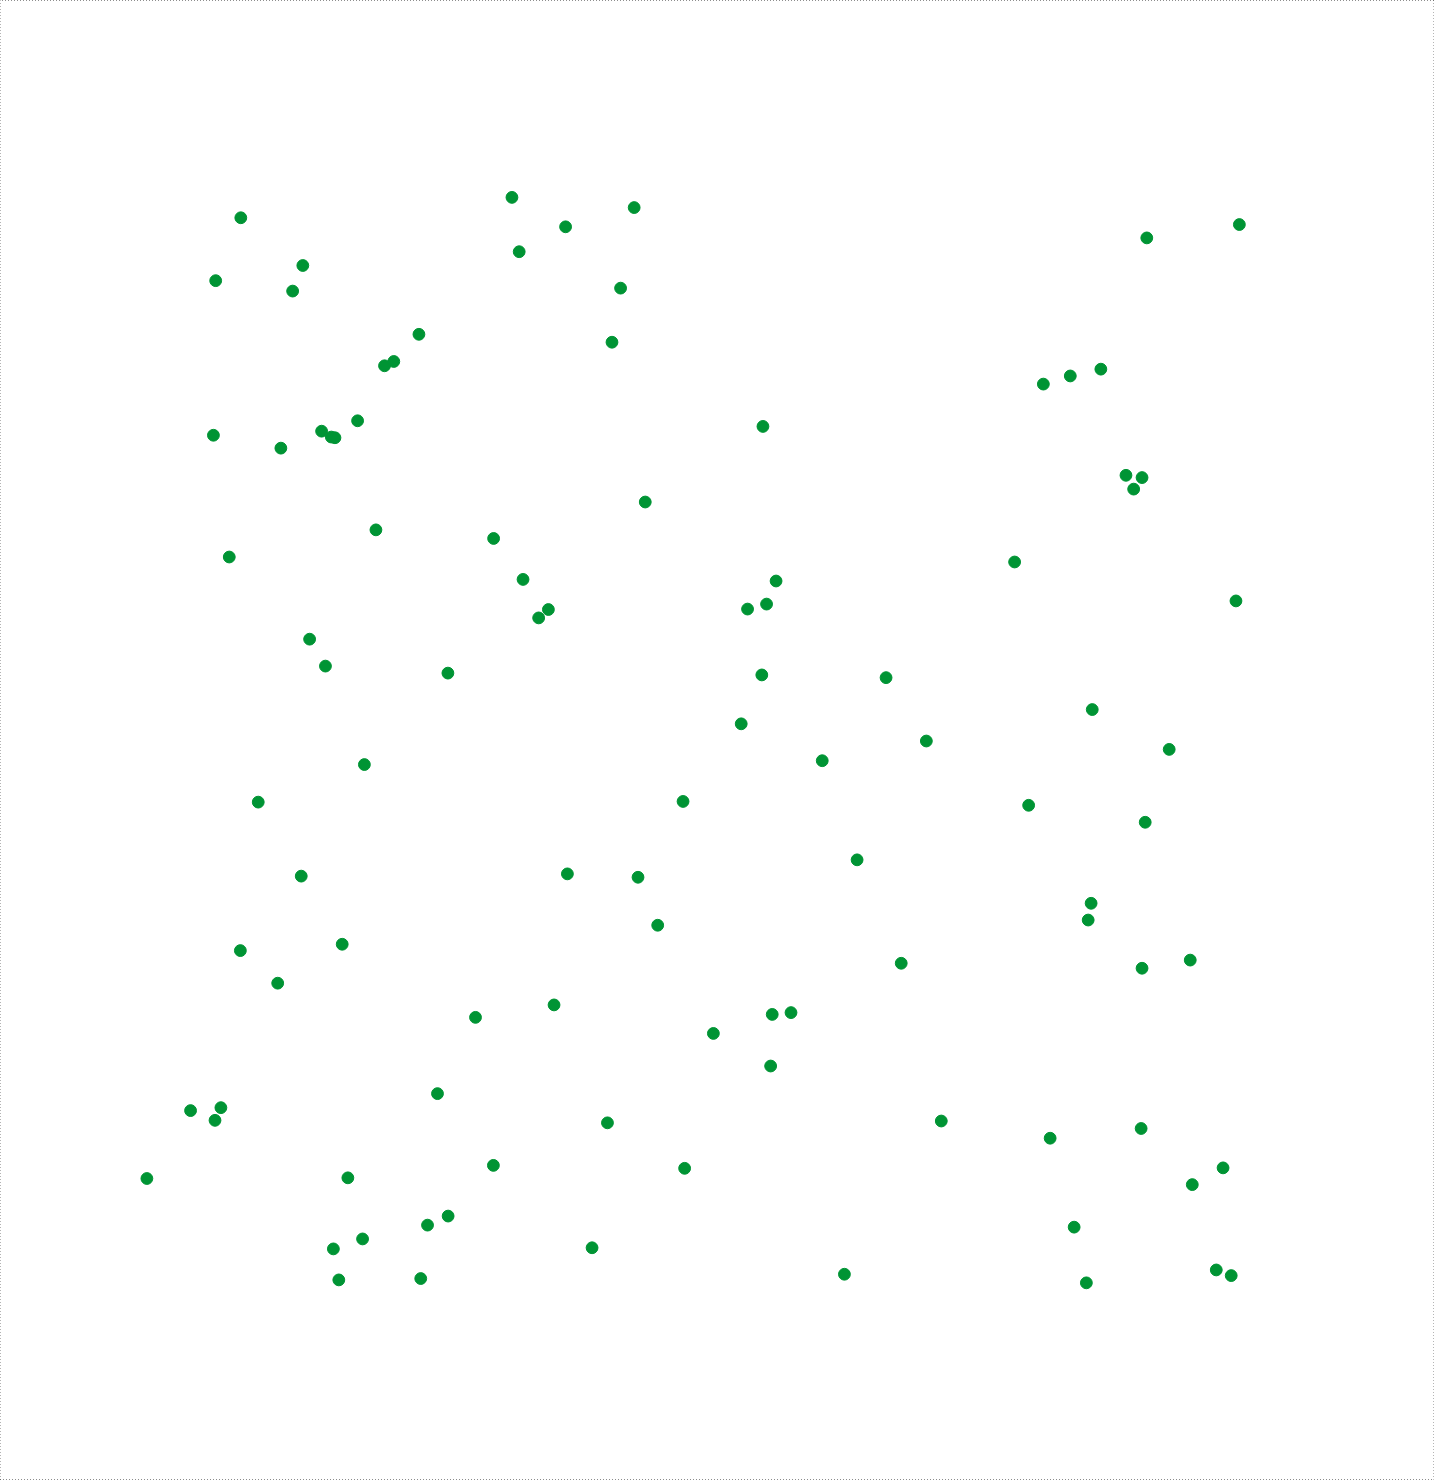
\includegraphics[width=0.55\textwidth]{figures/psi0}
\end{frame}


\begin{frame}{PSI stages...}{Finding centres... [1020]}
    \centering
    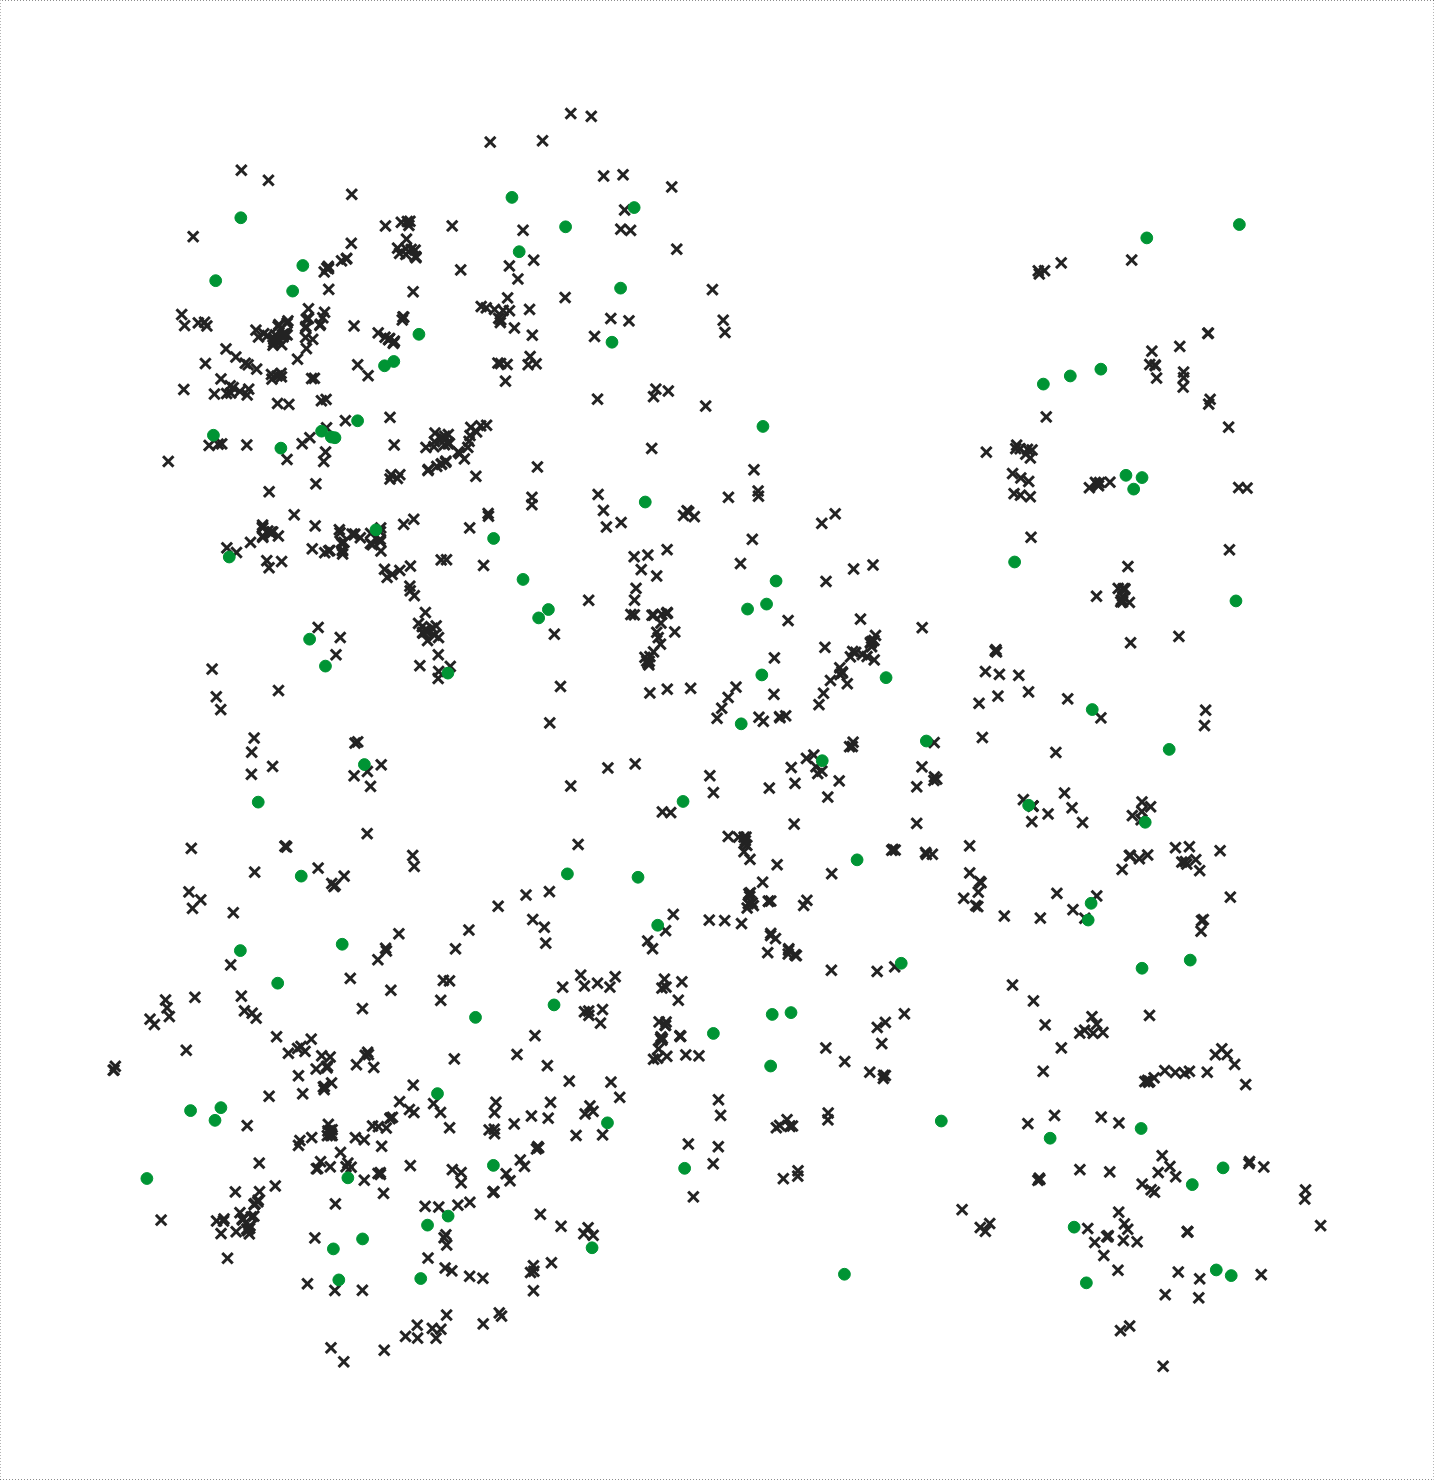
\includegraphics[width=0.55\textwidth]{figures/psi1}
\end{frame}

\begin{frame}{PSI stages...}{Finding candidates... [959]}
    \centering
    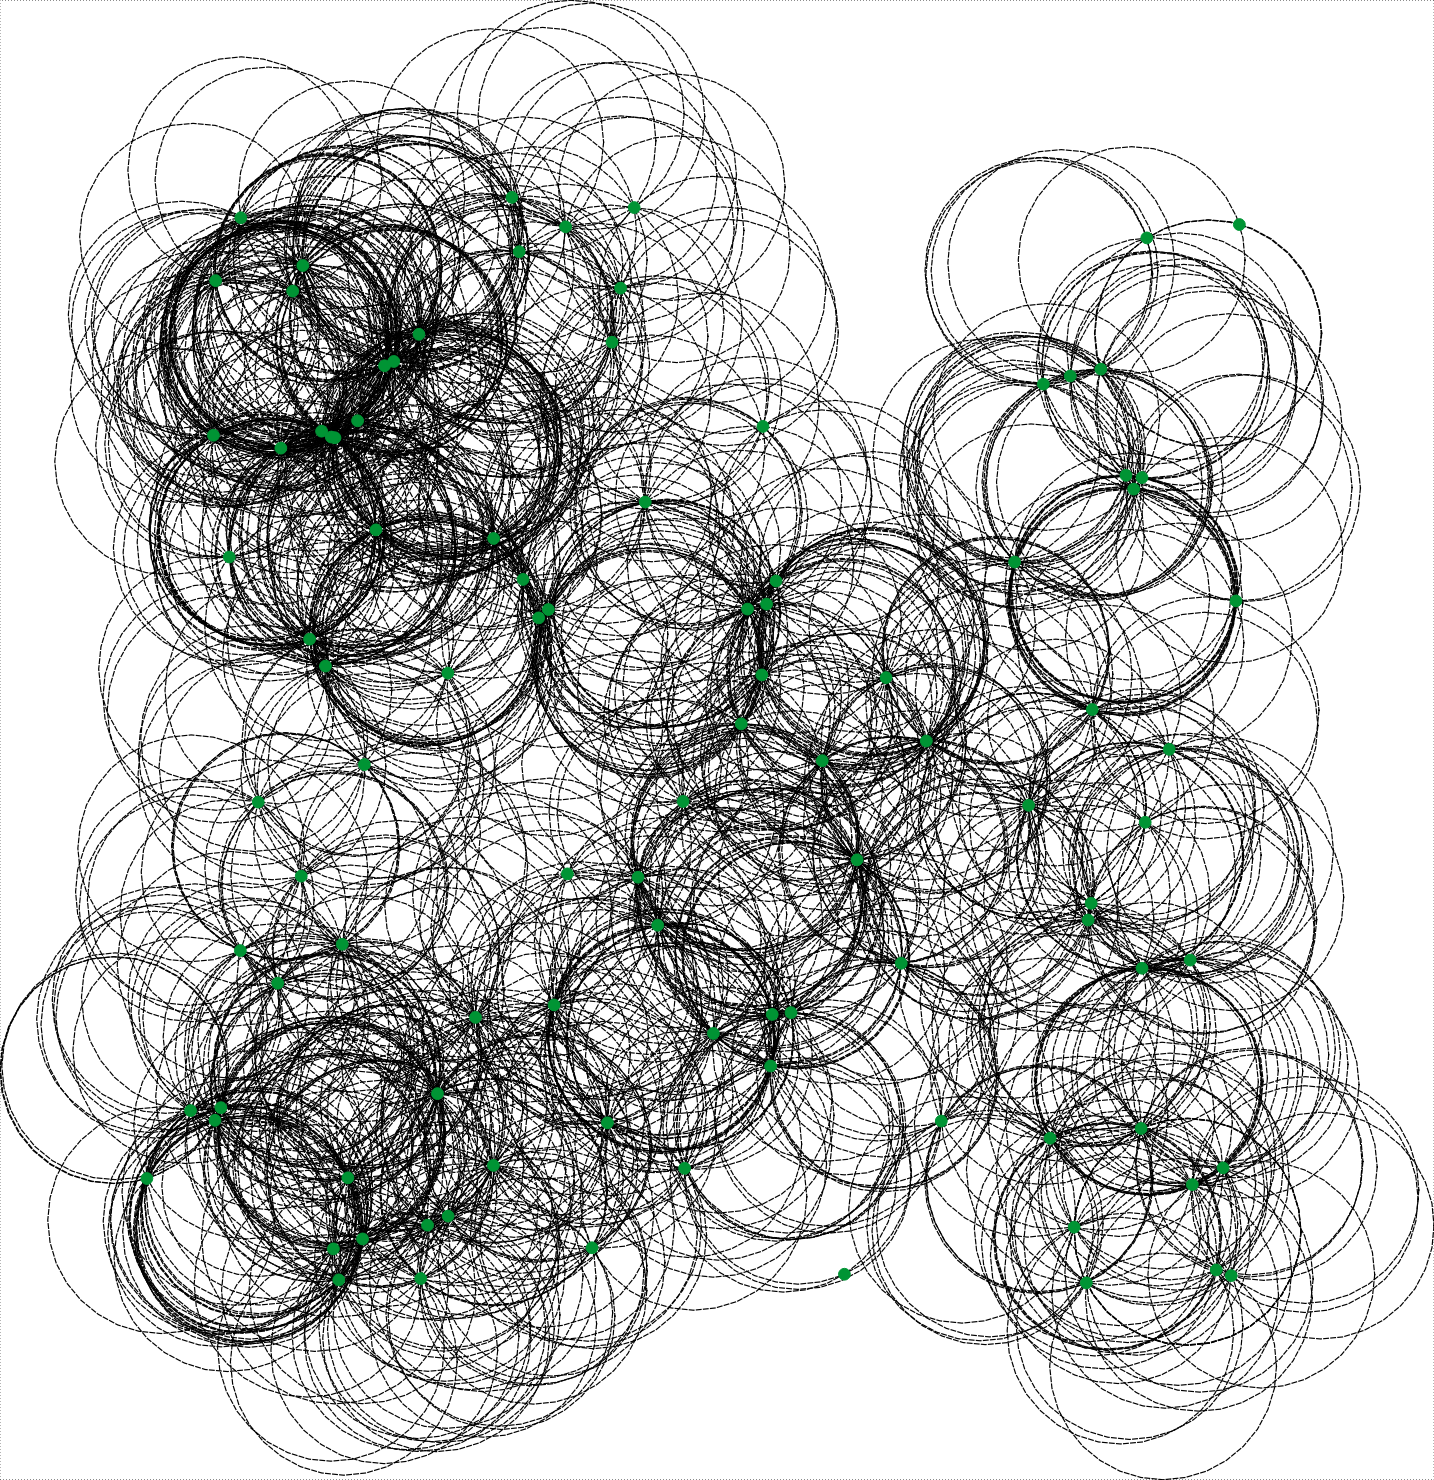
\includegraphics[width=0.55\textwidth]{figures/psi2}
\end{frame}

\begin{frame}{PSI stages...}{Finding active boxes... [88]}
    \centering
    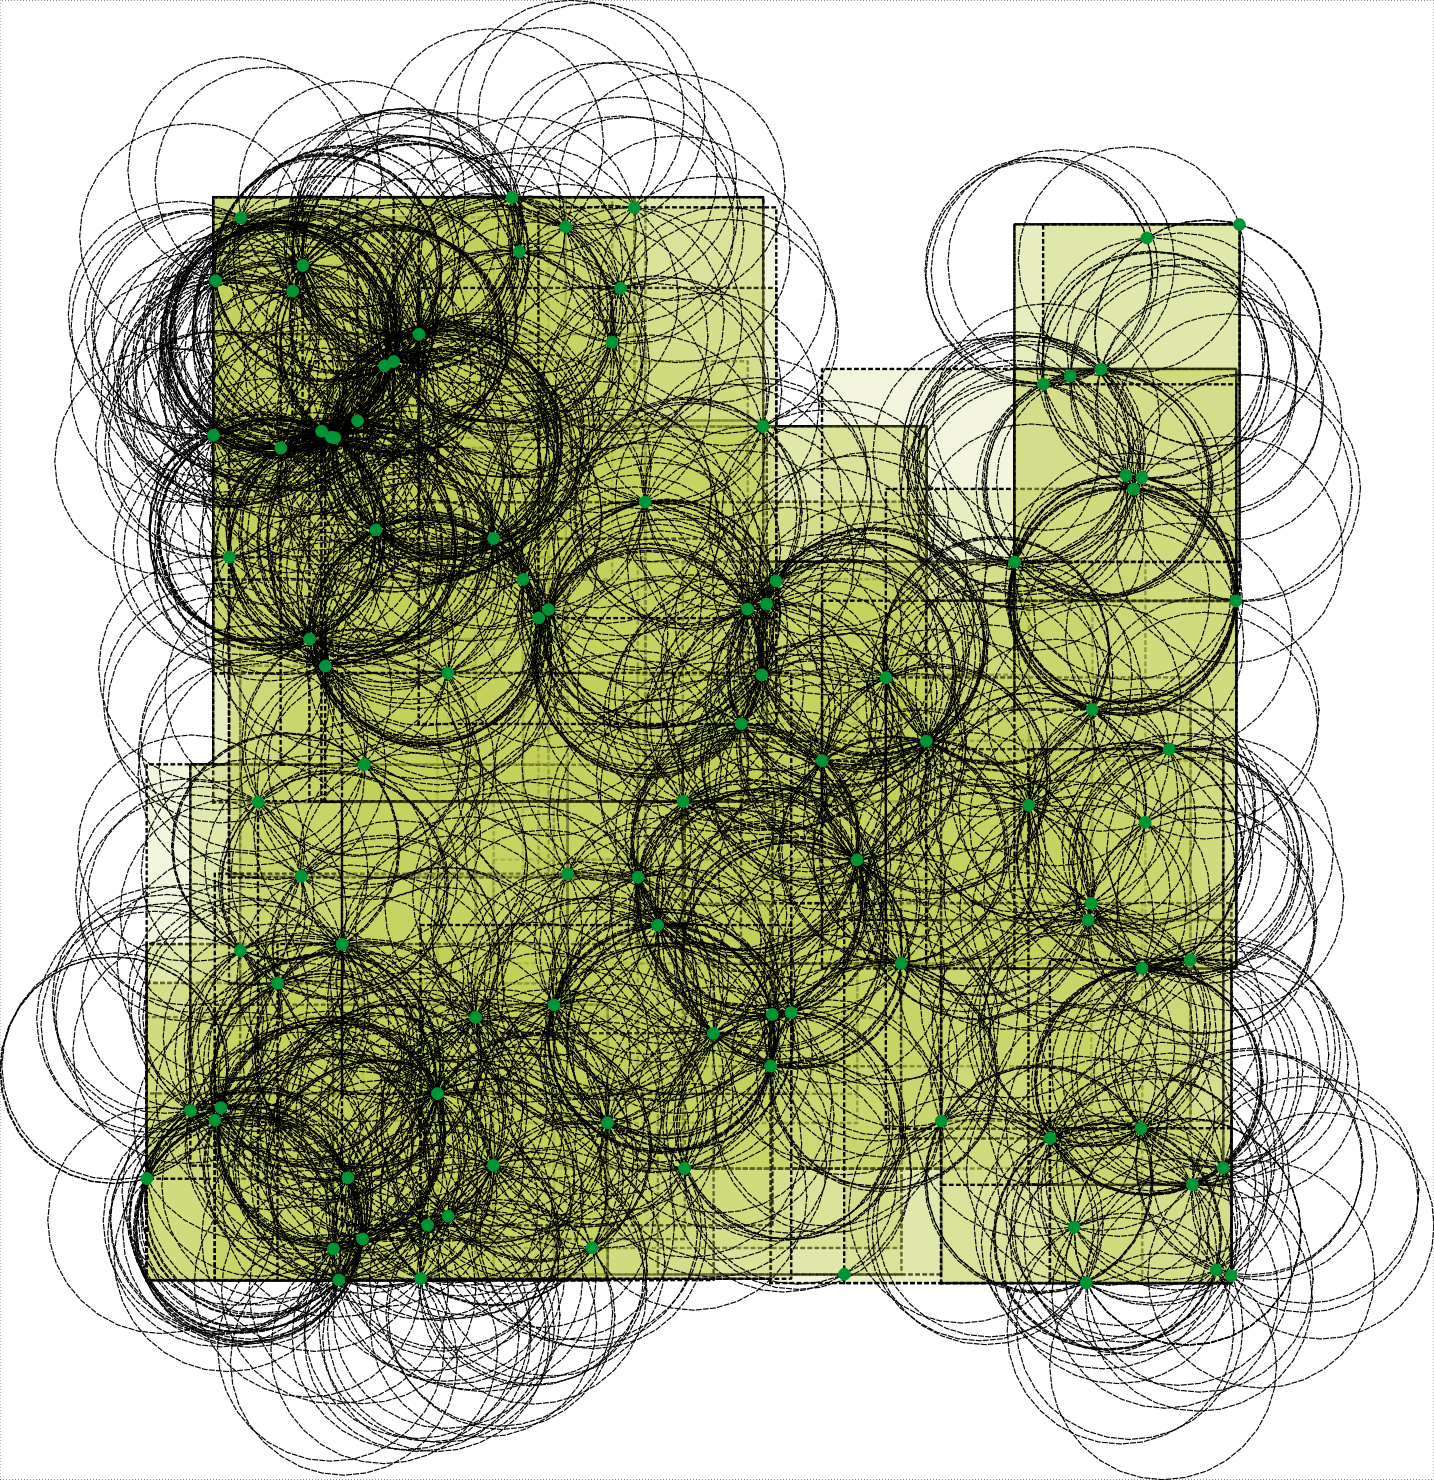
\includegraphics[width=0.55\textwidth]{figures/psi3}
\end{frame}

\begin{frame}{PSI stages...}{Updating disks in boxes...}
    \centering
    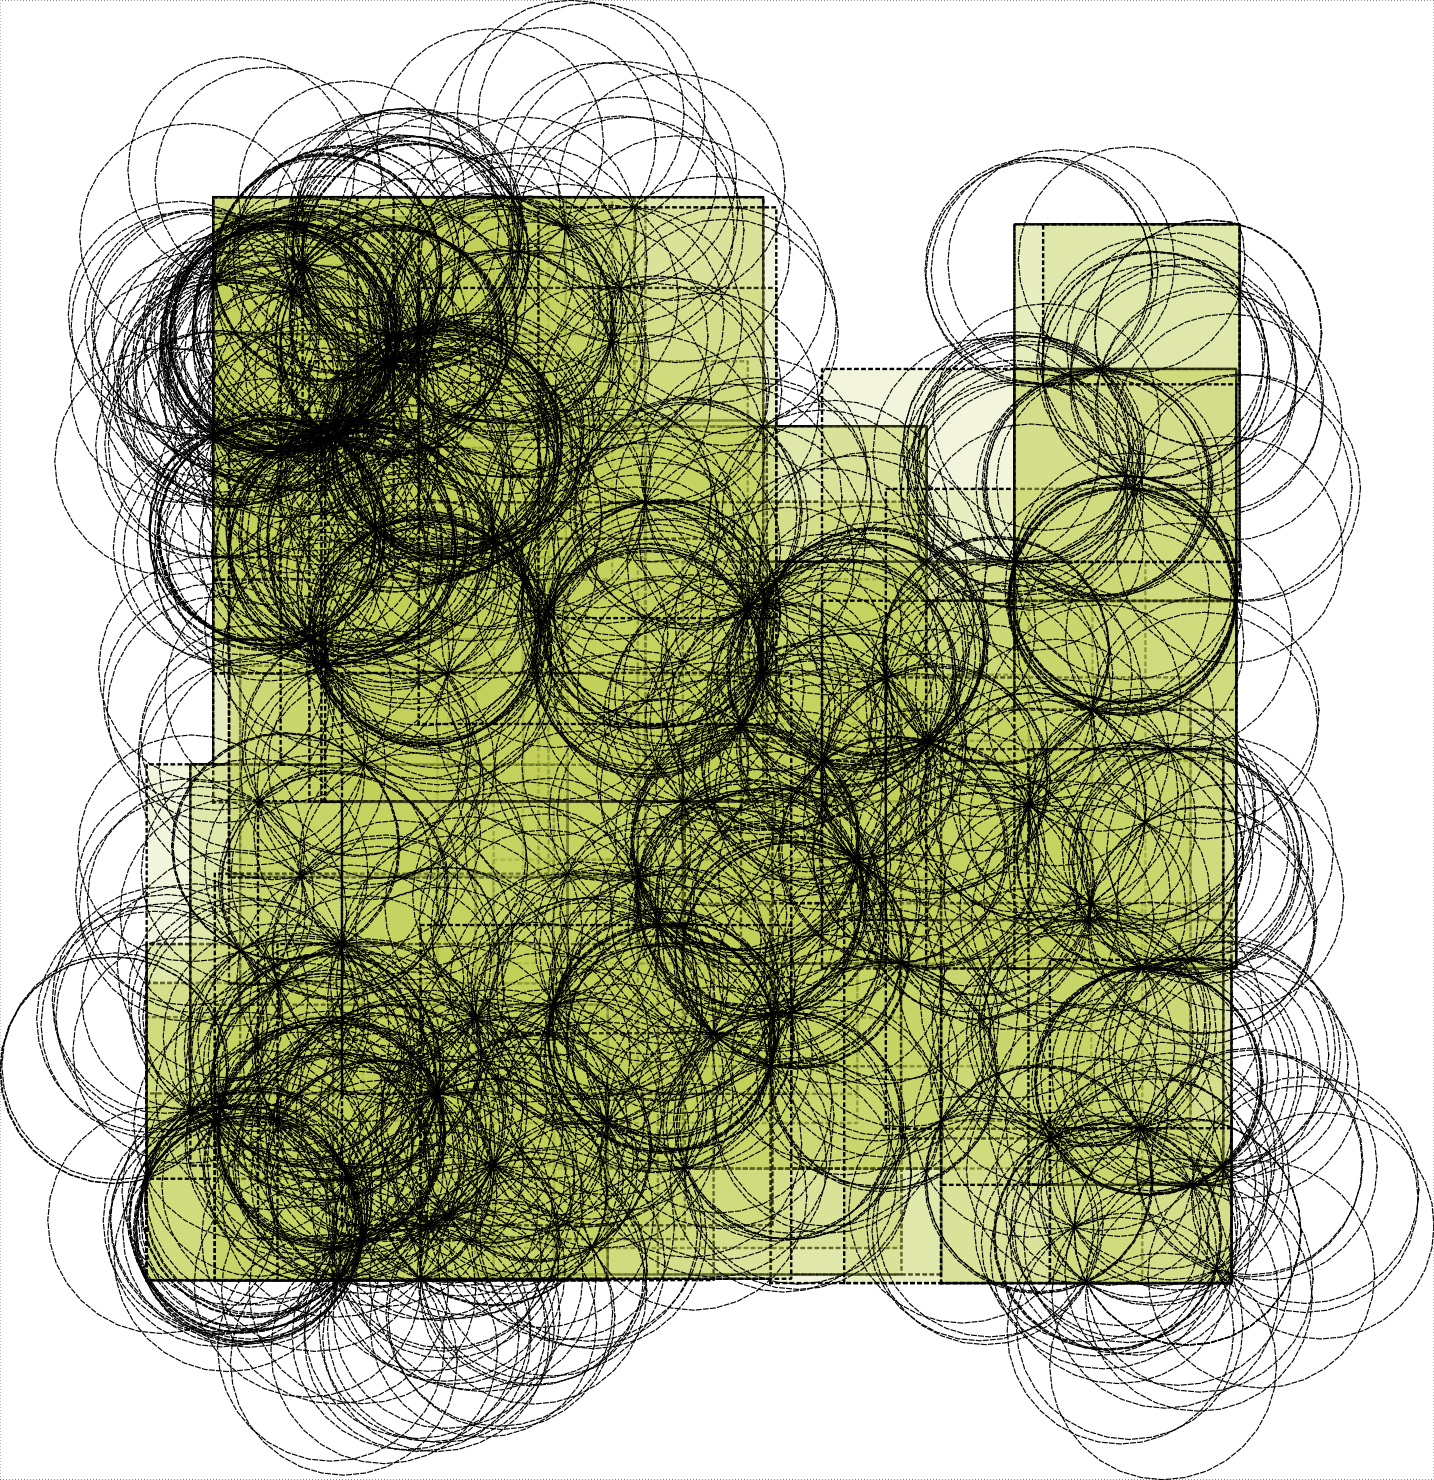
\includegraphics[width=0.55\textwidth]{figures/psi4}
\end{frame}

\begin{frame}{PSI stages...}{Updating disks in boxes...}
    \centering
    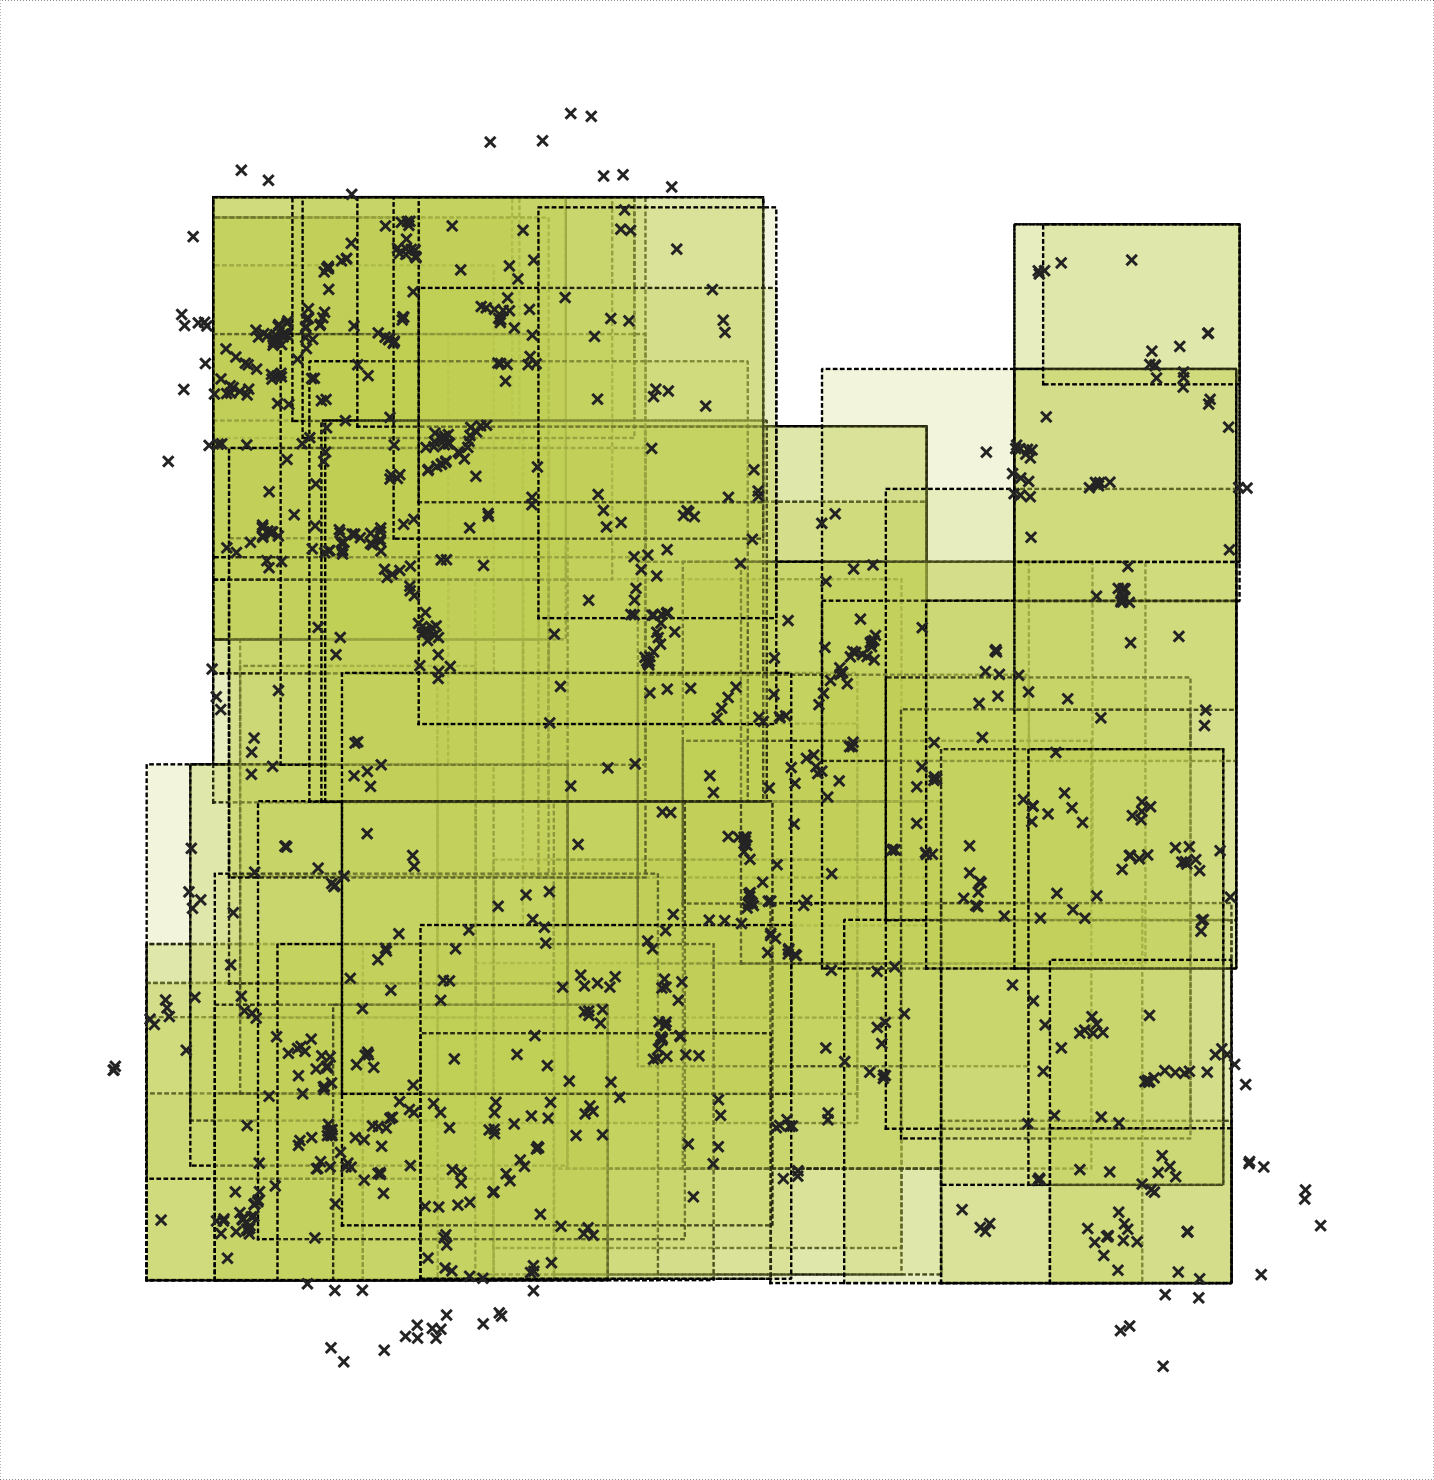
\includegraphics[width=0.55\textwidth]{figures/psi5}
\end{frame}

\begin{frame}{PSI stages...}{Running filterCandidates algorithm... [98]}
    \centering
    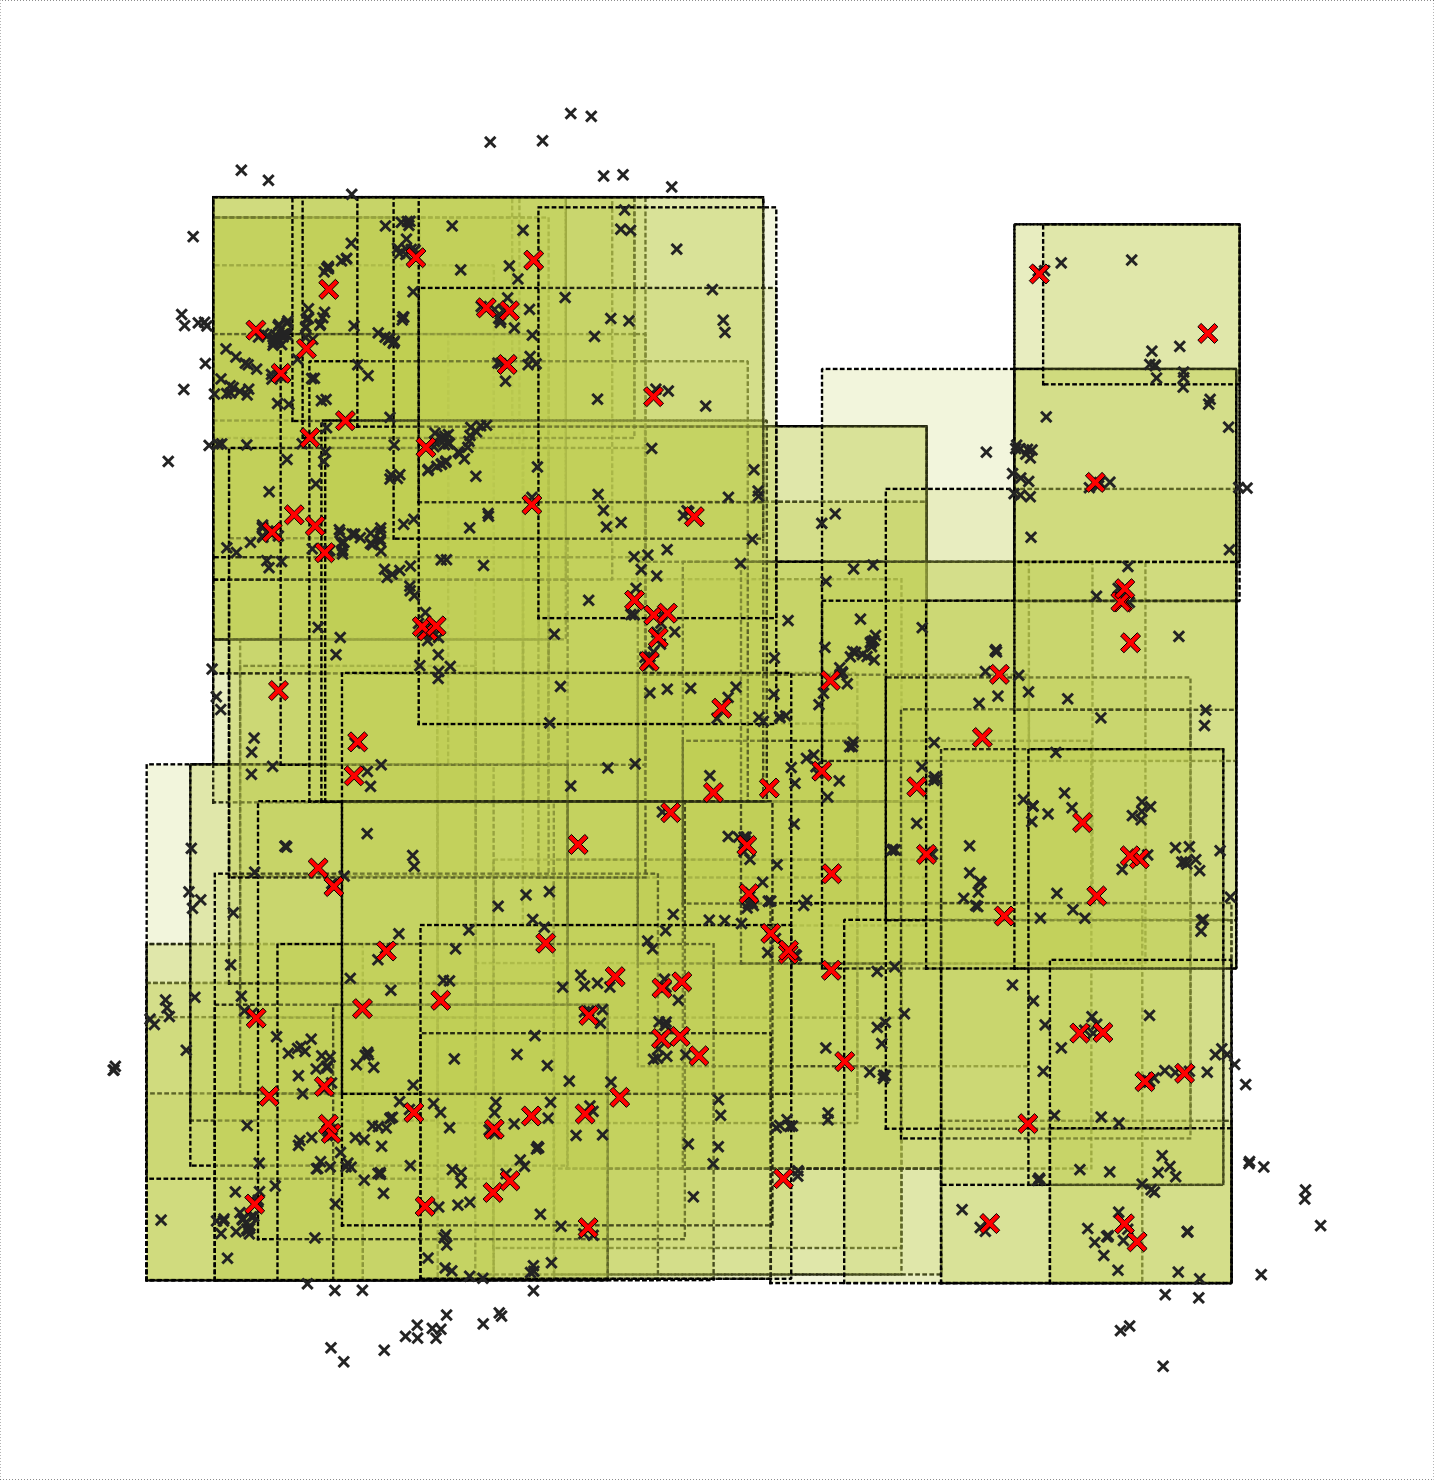
\includegraphics[width=0.55\textwidth]{figures/psi6}
\end{frame}

\begin{frame}{PSI results...}{Maximal disks in PSI...}
    \centering
    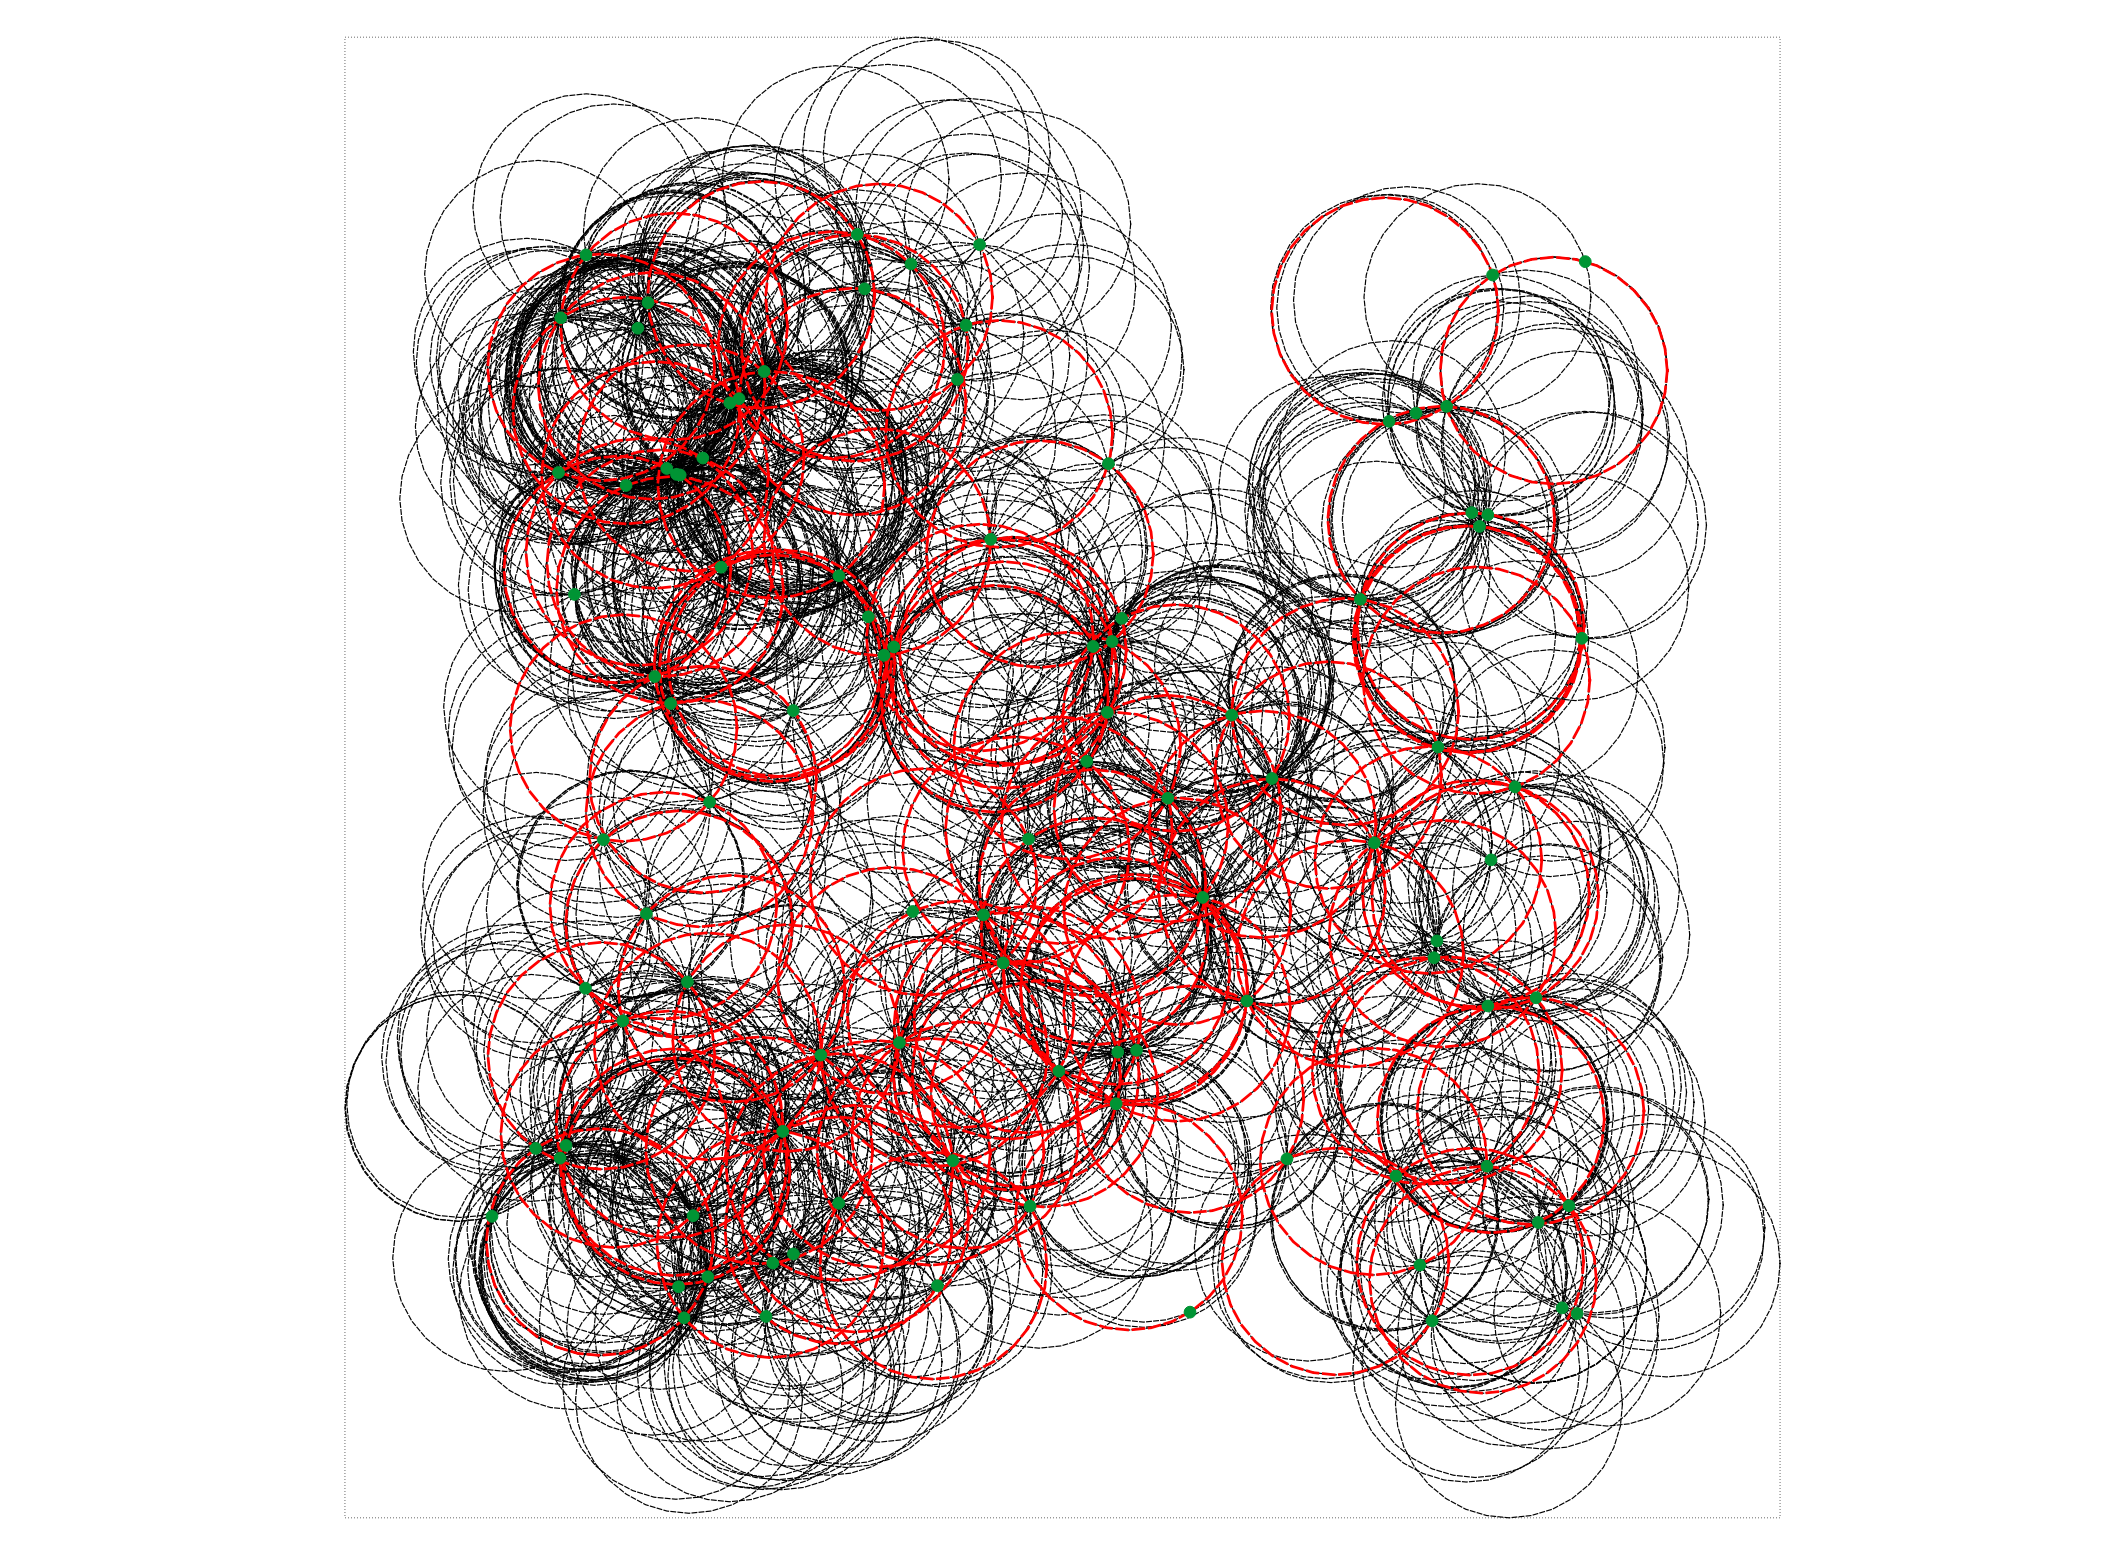
\includegraphics[width=0.75\textwidth]{figures/psi7}
\end{frame}

\begin{frame}{PSI results...}{Maximal disks in BFE...}
    \centering
    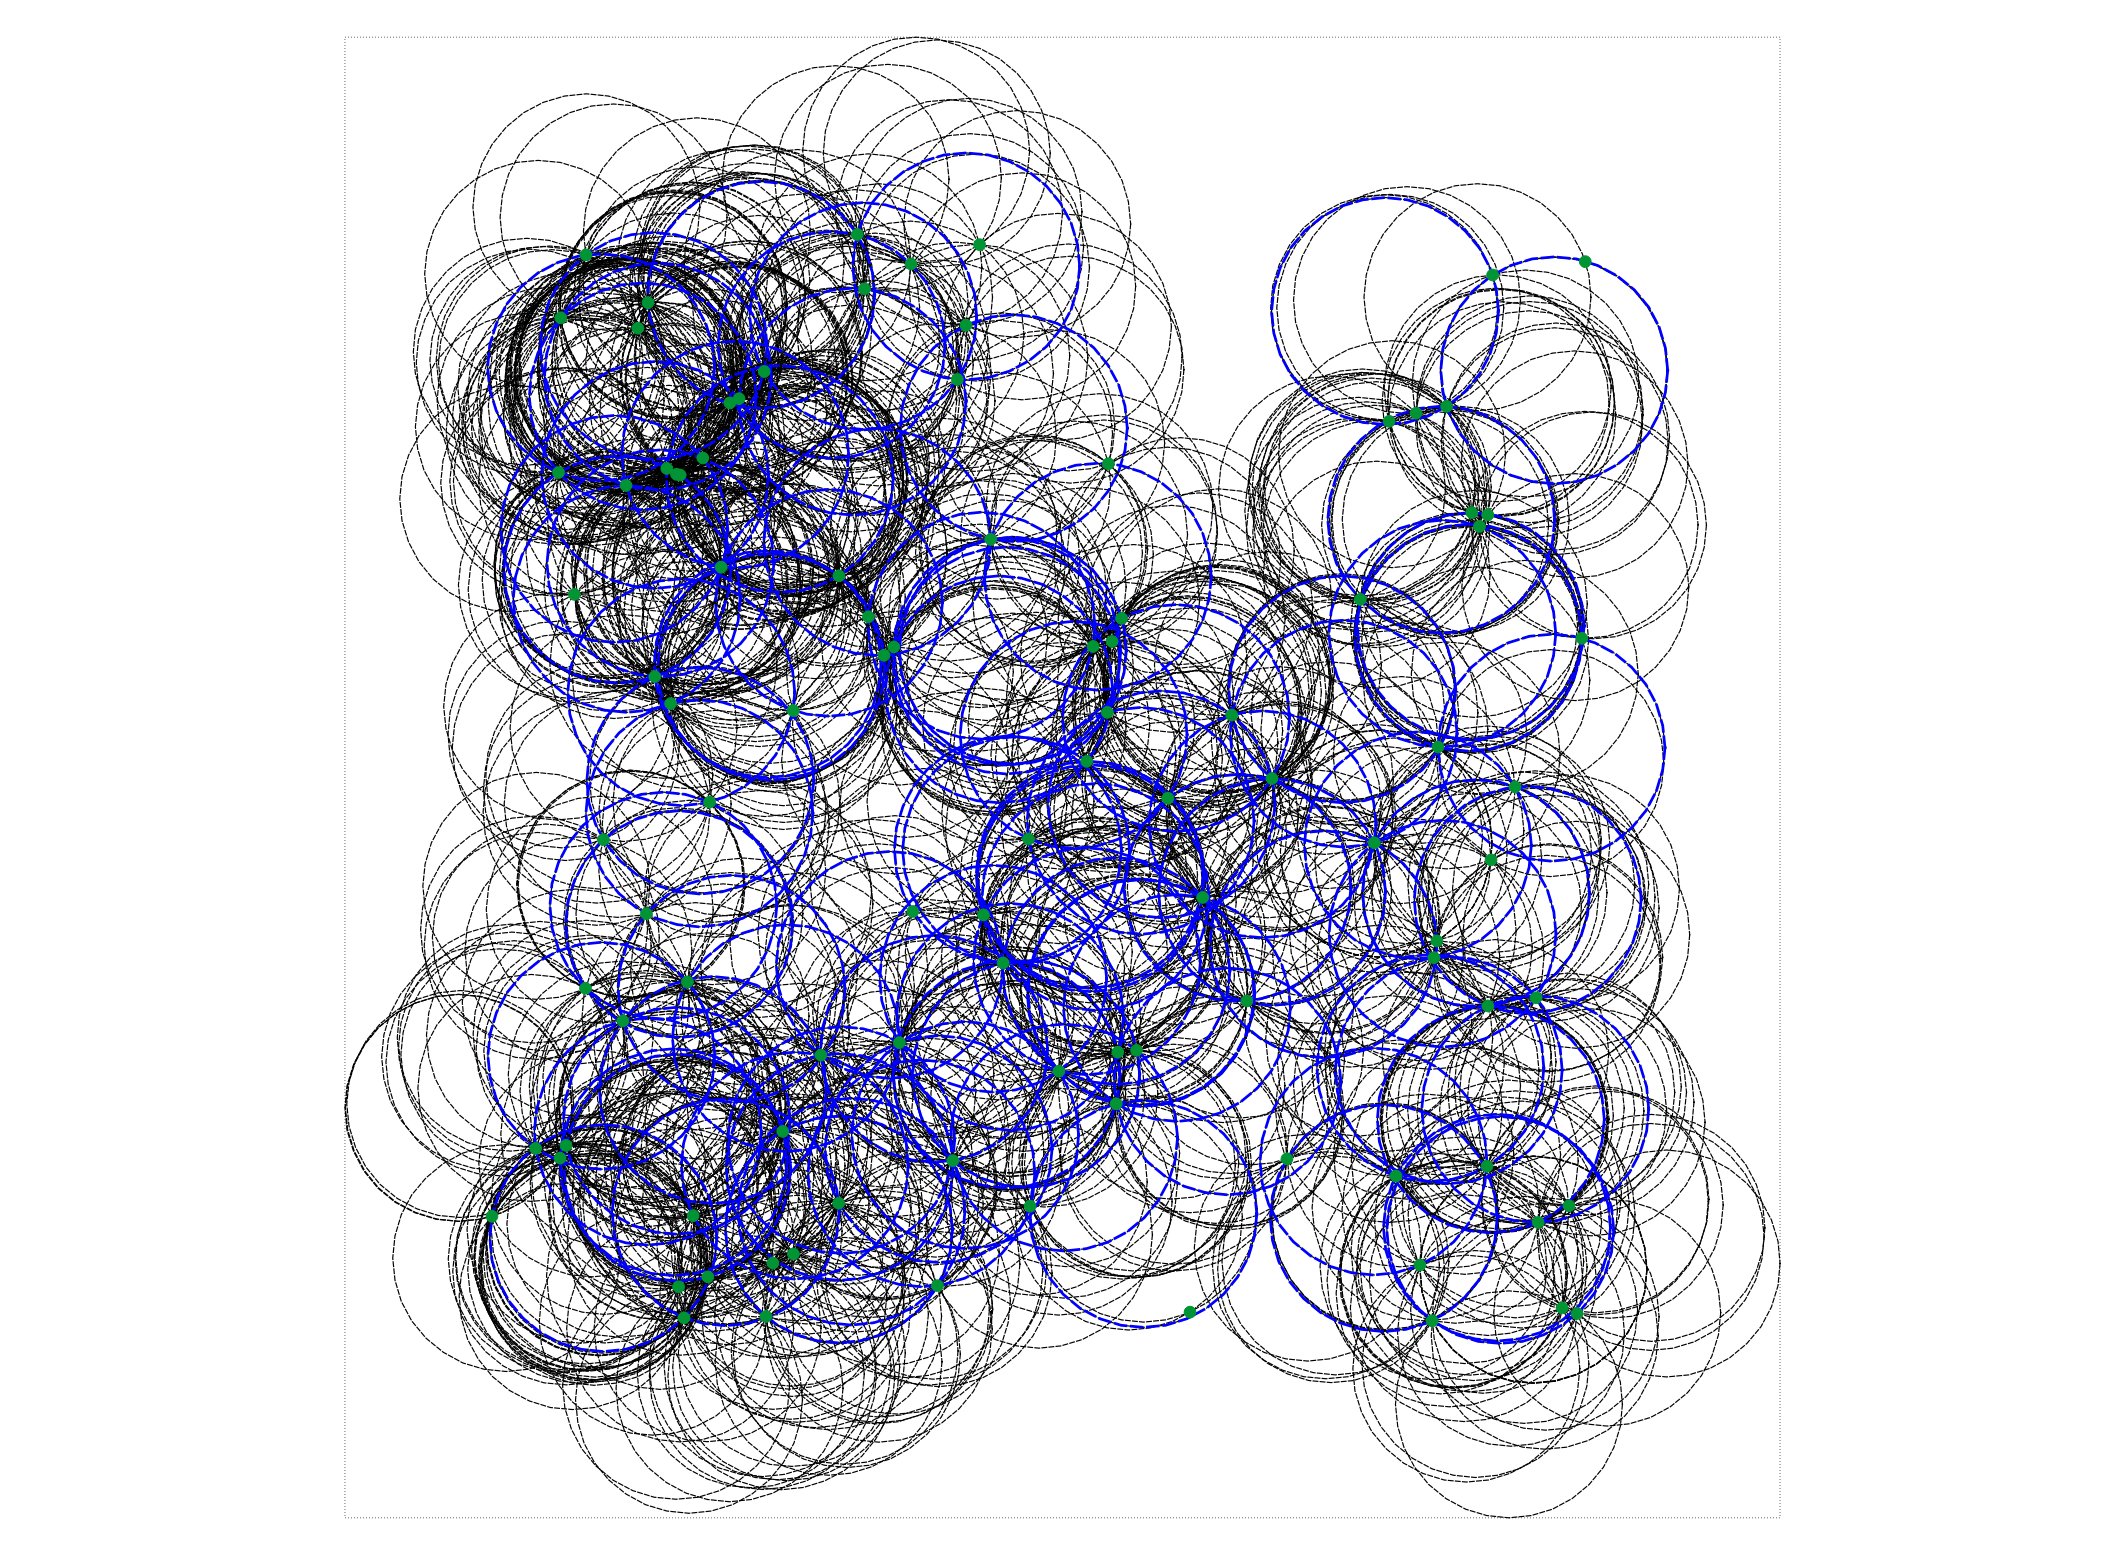
\includegraphics[width=0.75\textwidth]{figures/psi8}
\end{frame}

\begin{frame}{PSI and BFE...}
    \centering
    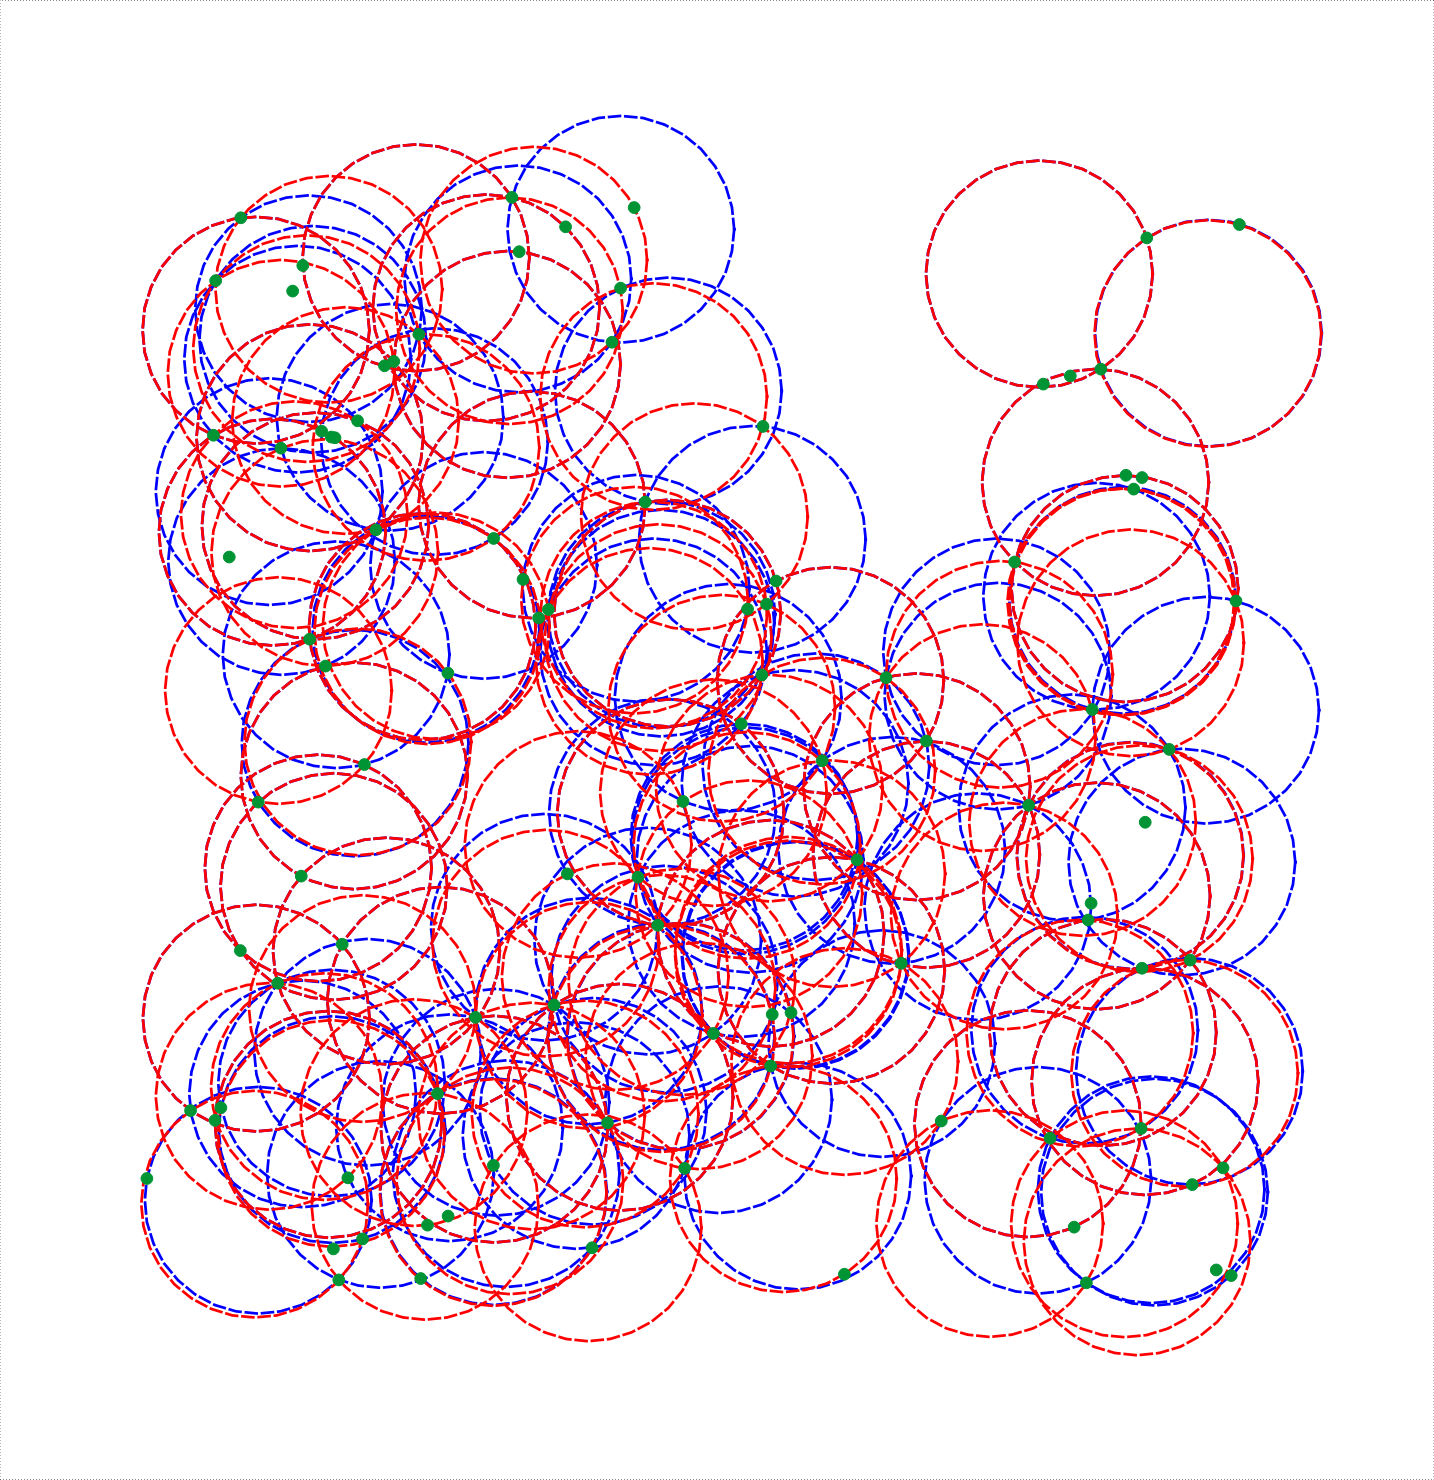
\includegraphics[width=0.6\textwidth]{figures/psi9}
\end{frame}

\begin{frame}{What's next?}
  \begin{itemize}
          \item Run performance experiments using BFE and PSI for dense datasets en parallel...
          \item Router, Resampler and Reprojector (RRR) are ready for ny\_taxis and ny\_bikes.
          \item Run RRR in new dataset sf\_taxis (San Francisco taxis)...
          \item Start working on temporal dimension...
          \begin{itemize}
                  \item Explore 3D partitioners...
          \end{itemize}
  \end{itemize}

\end{frame}

\end{document}

